\section{Relação Rastreamento e Reconhecimento}
\label{sec:rastreamento-reconhecimento}

	Até então, foi descrito como os Módulos de Rastreamento e de Reconhecimento funcionam de maneira isolada. Entretando, eles operam em conjunto. O Módulo de Rastreamento detém as informações sobre todos os usuários rastreados no ambiente e é responsável por requisitar identificação ao Módulo de Reconhecimento. Isto acontece sempre que um novo usuário for detectado ou quando for necessário reconhecer novamente um usuário já rastreado.

	% Basicamente, quando um novo usuário for detectado, a relação entre rastreamento e reconhecimento acontecerá de acordo com as etapas descritas na Figura~\ref{fig:rastreamento-reconhecimento}.

	Quando um novo usuário for detectado, o Módulo de Rastreamento obtém 20 imagens de cor sucessivas deste usuário. Para cada imagem, ele cria uma nova imagem composta somente pela região em que este usuário se encontra, como mostrado na Figura~\ref{fig:users-img}, e a envia ao Módulo de Reconhecimento requisitando identificação ao mesmo. O Módulo de Reconhecimento, por sua vez, realiza o reconhecimento facial e retorna ao Módulo de Rastreamento o nome do usuário e a confiança obtida. A cada 0.5 segundos, o Módulo de Reconhecimento verifica se chegou algum resultado de identificação. Caso tenha chegado, o Módulo de Rastreamento computa o resultado e decide qual identidade será atribuída ao respectivo usuário. A Figura~\ref{fig:rastreamento-reconhecimento} ilustra esta relação entre os dois módulos.

		\begin{figure}[htb]
			\begin{center}
				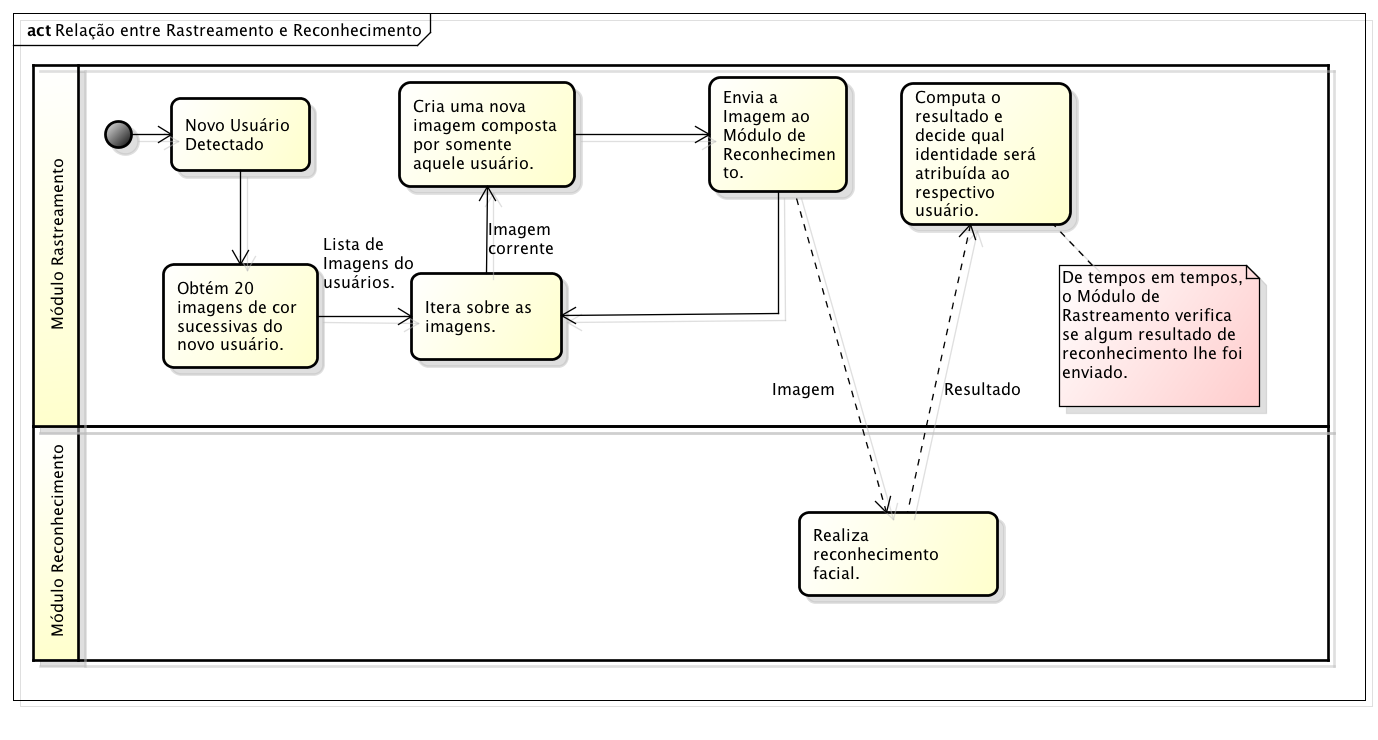
\includegraphics[scale=0.5]{figuras/4.ProblemaEProposta/diagrama-relacao.png}
			\end{center}
			\caption{Representação da relação que o Módulo de Rastreamento terá com o Módulo de Reconhecimento quando um novo usuário for detectado.}
			\label{fig:rastreamento-reconhecimento}
		\end{figure}
	
		% \begin{enumerate}
		%  	\item O Módulo de Rastreamento detecta novo usuário, e obtém um número pré-definido de imagens sucessivas do novo usuário. Para cada imagem, ele cria uma nova imagem de cor contendo somente aquele usuário, como mostrado na Figura (\textbf{colocar a figura aqui}), e a envia para o Módulo de Reconhecimento.
		%  	\item Para cada imagem recebida, o Módulo de Reconhecimento tenta reconhecer o novo usuário e retorna ``vazio'' ou o nome e a confiança do reconhecimento.
		%  	\item O Módulo de Rastreamento verifica se a confiança é maior que um limiar pré-definido, se for ele incrementa o contador que armazena o número de vezes que o usuário foi reconhecido, armazena o nome obtido juntamente com a confiança e calcula qual nome  será atribuído ao novo usuário. Esse cálculo será feito por meio de uma média ponderada utilizando os diferentes resultados obtidos por cada reconhecimento e suas respectivas confianças.
	 % 	\end{enumerate} 
	
	Ao invés de realizar o reconhecimento somente quando novos usuários são detectados, com o objetivo de melhorar a confiança no reconhecimento, o Sistema TRUE realiza continuamente a identificação dos usuários já reconhecidos. Essas tentativas de reconhecer novamente os usuários ocorrerão a cada 5 segundos seguindo as mesmas etapas de quando um novo usuário for detectado. A única etapa que se difere é a primeira, ou seja, ao invés de obter várias imagens de um mesmo usuário, é obtida uma imagem de cada usuário rastreado e a mesma é enviada ao Módulo de Reconhecimento.

	Como visto na Figura~\ref{fig:rastreamento-reconhecimento}, ao obter um resultado de reconhecimento para determinado usuário, o Módulo de Rastreamendo deve computar qual identidade será atribuída ao mesmo. Para isso, este módulo mantém para cada usuário o número total de vezes que este já foi reconhecido, os diferentes nomes obtidos pelo Módulo de Reconhecimento bem como a confiança média para cada nome e o número de vezes que cada nome foi atribuído àquele usuário. Com todos esses dados, a identidade do usuário é definida por meio de uma média ponderada entre as confianças de cada nome, onde os pesos utilizados são compostos pelo número de vezes que o respectivo nome foi atribuído ao usuário. O exemplo a seguir aprensenta em detalhes como a identidade de um usuário é definida.

	\begin{description}
 		João é um usuário do ambiente inteligente que está sendo rastreado há algum tempo e que já foi reconhecido algumas vezes. Como já mencionado, o Módulo de Rastreamento mantém para cada usuário o número total de vezes que este já foi reconhecido, os diferentes nomes obtidos pelo Módulo de Reconhecimento bem como a confiança média para cada nome e o número de vezes que cada nome foi atribuído àquele usuário. Neste caso, a Tabela~\ref{tab:joao} mostra os dados mantidos para o usuário João pelo Módulo de Rastreamento, em que ``João'', ``Danilo'' e ``Tales'' são as identidades que já foram obtidas ao se tentar reconhecer o João. A segunda coluna desta tabela mostra a confiança média do reconhecimento para cada nome e a última mostra o número de vezes que cada nome foi atribuído a João.

 		% No momento, o Módulo de Rastreamento mantém vários dados sobre o João descritos na Tabela~\ref{tab:joao}. Como já mencionado, o Módulo de Rastreamento Então, para computar qual identidade será atribuída ao usuário, o Módulo de Rastreamento realiza os cálculos~\ref{eq:joao}. Como o resultado da média ponderada se aproxima mais da confiança do nome João, este foi escolhido como sendo sua identidade.
	\end{description}

	\begin{table}[htb]
		\begin{center}
			\caption{Exemplos de dados de reconhecimento mantidos para cada usuário rastreado pelo Módulo de Rastreamento.}
			\label{tab:joao}
			\begin{tabular}{|c|c|c|}
				\hline \bf Nome & Confiança Média & Número de Vezes \\
				\hline \hline \bf João & 0.947302 & 15 \\
				\hline \bf  Danilo & 0.934010 & 1 \\
				\hline \bf Tales & 0.950320 & 3 \\
				\hline
				\hline \multicolumn{2}{|c|}{\bf Total}  & 19 \\
				\hline
			\end{tabular}
		\end{center}
	\end{table}

	\begin{align}
		\label{eq:joao}
		M_p = \frac{15 * 0.947302 + 1 * 0.934010 + 3 * 0.950320}{19} = 0.947079
	\end{align}

	\begin{align}
	\nonumber & Joao: 0.947079 - 0.947302 = -0.000223\\
		\nonumber & Danilo: 0.934010 - 0.947302 = -0.013292\\
		\nonumber & Tales: 0.950320 - 0.947302 = 0.003018
	\end{align}

	Com todos esses dados de reconhecimento, além dos dados de rastreamento e localização de cada usuário, o Módulo de Rastreamento consegue centralizar todas as informações necessárias de cada usuário. A Figura~\ref{fig:truetotal} exemplifica um usuário rastreado pelo Sistema TRUE onde as informações de localização e identificaçao estão presentes.

	\begin{figure}[htb]
			\begin{center}
				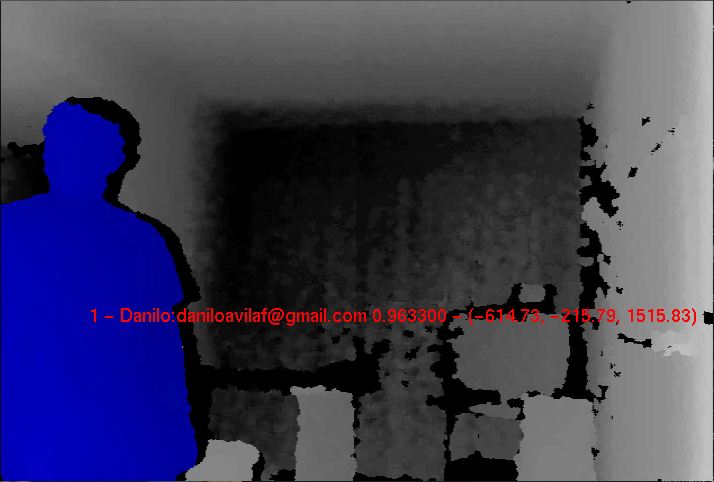
\includegraphics[scale=0.5]{figuras/4.ProblemaEProposta/user-reconhecido.png}
			\end{center}
			\caption{Exemplo de um usuário rastreado e identificado pelo Sistema TRUE.}
			\label{fig:truetotal}
		\end{figure}

